\documentclass[aspectratio=169,10pt]{beamer}
\usepackage[T1]{fontenc}
\usepackage[utf8]{inputenc}
\usepackage[english]{babel}
\usepackage{lmodern}
\usepackage{amsmath,amssymb,booktabs,graphicx}
\usetheme{Madrid}
\definecolor{navy}{RGB}{22,50,79}
\definecolor{teal}{RGB}{8,126,139}
\setbeamercolor{structure}{fg=navy}
\setbeamercolor{frametitle}{bg=navy,fg=white}
\setbeamercolor{block title}{bg=teal,fg=white}
\setbeamertemplate{navigation symbols}{}
\setbeamertemplate{footline}[frame number]
\setbeamertemplate{itemize items}[circle]
\graphicspath{{assets/}}
\setbeameroption{hide notes}
\title{MNIST MLP from Scratch}
\subtitle{Learning neural network foundations with Python and NumPy}
\author{}
\date{16 November 2026}
\begin{document}
\begin{frame}\titlepage\note{30 seconds. Explain that the talk has three parts: the basic idea, the dataset, and what we built. No prior machine learning background is needed.}\end{frame}
\section{Part 1: Understanding Neural Networks}
\begin{frame}{Learning from examples}
\begin{itemize}
\item A neural network is a mathematical model that finds patterns in data.
\item It receives information and produces a prediction.
\item In supervised learning, examples include the answer we want it to learn.
\end{itemize}

\note{Suggested speaking time: 75 seconds. Use a general example: classify fruit using measurements such as color and size. Ask which measurements might help distinguish an apple from a pear. Explain that people supply the examples, while the model adjusts its numerical settings.}
\end{frame}

\begin{frame}{Why call it a neuron?}
\begin{itemize}
\item The name is inspired by how biological neurons receive and pass on signals.
\item An artificial neuron receives numbers, combines them, and passes on a result.
\item It is a simple analogy: this model does not reproduce how a brain works.
\end{itemize}

\note{Suggested speaking time: 60 seconds. Describe three actions: receive, combine, pass on. Avoid anatomical detail or claims that the network thinks like a person.}
\end{frame}

\begin{frame}{Weights: giving different influence to inputs}
\begin{exampleblock}{Illustrative weighted score}\[2\times0.2+1\times0.6+0.1=1.1\]\end{exampleblock}\begin{itemize}
\item A weight controls how much an input contributes to the result.
\item A bias is an extra adjustment added to that combination.
\item The model changes these values during learning.
\end{itemize}

\note{Suggested speaking time: 75 seconds. Relate weights to a weighted score, but explain that weights need not add to one and can be negative. Walk through the illustrative arithmetic. It is not a probability or a real fitted model.}
\end{frame}

\begin{frame}{Layers: combining information in stages}
\begin{center}\Large Inputs $\rightarrow$ Layers $\rightarrow$ Prediction\end{center}\medskip \begin{itemize}
\item Several artificial neurons form a layer.
\item Each layer uses the results of the previous layer.
\item This sequence of calculations is called the forward pass.
\end{itemize}

\note{Suggested speaking time: 80 seconds. Use the diagram as a verbal route. A hidden layer is simply a stage between the input and output, not something mysterious or conscious.}
\end{frame}

\begin{frame}{ReLU: a simple rule inside a layer}
\begin{center}\Large $-3\mapsto0\qquad0\mapsto0\qquad4\mapsto4$\end{center}\medskip \begin{itemize}
\item An activation function transforms a neuron's numerical result.
\item ReLU keeps positive values and replaces negative values with zero.
\item Using such rules lets a network represent more complex patterns.
\end{itemize}

\note{Suggested speaking time: 65 seconds. Read each example aloud and ask what ReLU would do to zero. No derivative or matrix explanation is needed. The point is that a network applies simple operations repeatedly.}
\end{frame}

\begin{frame}{Softmax: comparing possible answers}
\begin{exampleblock}{Example output}\centering A: 65\%\qquad B: 25\%\qquad C: 10\%\end{exampleblock}\begin{itemize}
\item The final layer produces a score for each possible class.
\item Softmax converts those scores into values that sum to 100\%.
\item The predicted class is the one with the largest value.
\end{itemize}

\note{Suggested speaking time: 80 seconds. Use three generic classes A, B and C, not digit examples yet. Ask which class wins. Emphasize that these are model scores: a high score can still be wrong.}
\end{frame}

\begin{frame}{Measuring how wrong a prediction is}
\begin{itemize}
\item We compare the prediction with the known answer.
\item The loss is a number that describes the mismatch; lower is better.
\item Cross-entropy gives a larger penalty when the correct class receives a very low score.
\end{itemize}

\note{Suggested speaking time: 70 seconds. Contrast accuracy and loss using two correct predictions that give the correct class 90 percent and 60 percent. Both count as correct, but their losses differ. No logarithms are needed.}
\end{frame}

\begin{frame}{Using mistakes to improve the model}
\begin{itemize}
\item Backpropagation calculates how changes to each connection would affect the loss.
\item Gradient descent uses that information to make small adjustments.
\item The learning rate controls the size of those adjustments.
\end{itemize}

\note{Suggested speaking time: 90 seconds. Use the analogy of adjusting a recipe after tasting it: observe the result, identify which changes may help, then make a small adjustment. Clarify that the computer uses calculations, not understanding or taste. Very large adjustments can make the result worse.}
\end{frame}

\begin{frame}{The learning cycle}
\begin{itemize}
\item 1. Show examples and calculate predictions.
\item 2. Measure the loss and calculate useful adjustments.
\item 3. Change the weights slightly and repeat with more examples.
\end{itemize}

\note{Suggested speaking time: 80 seconds. Ask the audience to explain the cycle in their own words. Emphasize that the aim is to work on new examples, not only on the examples used for practice. Now introduce the dataset.}
\end{frame}

\section{Part 2: The MNIST Dataset}
\begin{frame}{Our task: recognize a handwritten digit}
\centering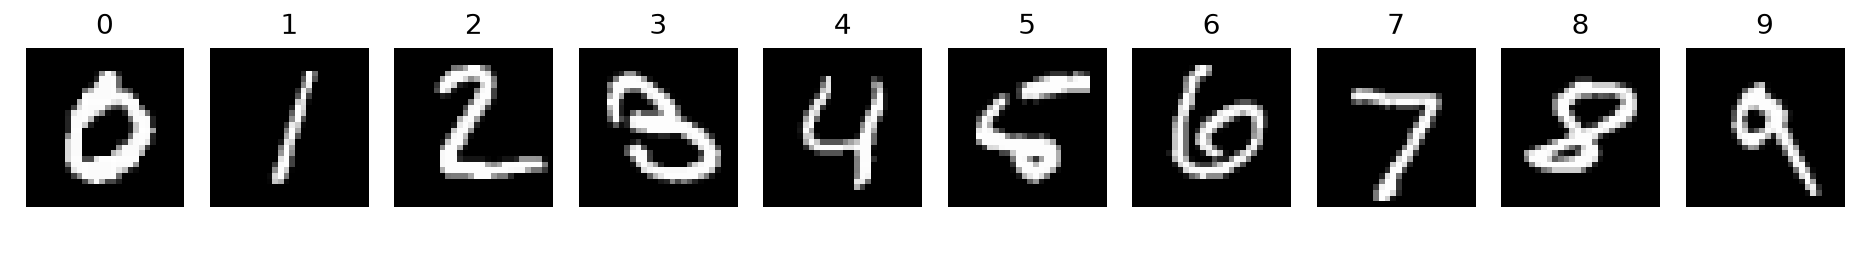
\includegraphics[width=\textwidth]{mnist.png}\par\raggedright \begin{itemize}
\item MNIST is a collection of small handwritten-digit images.
\item Each image has a label: the correct digit, from 0 to 9.
\item We use the images and labels to teach and evaluate the model.
\end{itemize}

\note{Suggested speaking time: 50 seconds. Point to two drawings that look different despite representing the same digit. Explain that variation in handwriting makes the task interesting. Attribute the dataset to LeCun, Cortes and Burges.}
\end{frame}

\begin{frame}{How an image becomes numbers}
\begin{center}\Large $28\times28=784$\end{center}\begin{itemize}
\item Each image has 28 rows and 28 columns: 784 pixels.
\item A pixel is a brightness measurement, not a complete drawing.
\item We read the pixels in a fixed order and divide by 255 to obtain values between 0 and 1.
\end{itemize}

\note{Suggested speaking time: 60 seconds. Explain black as zero, white as one, and gray as an intermediate value. Flattening changes the arrangement of values, not their content. The order must stay consistent.}
\end{frame}

\begin{frame}{Do we have examples of every digit?}
\centering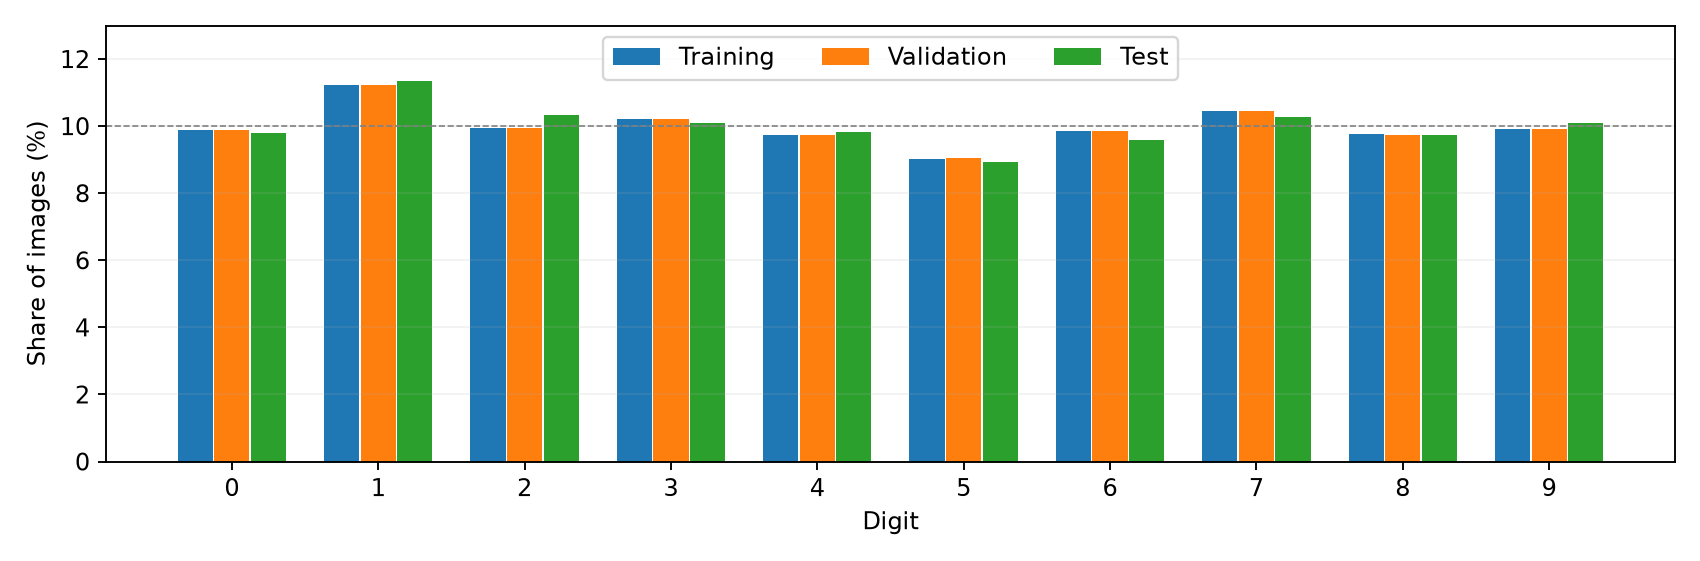
\includegraphics[width=.91\textwidth]{classes_en.png}\par\raggedright \begin{itemize}
\item Each digit represents roughly one tenth of the images.
\item The groups have slightly different sizes; they are not perfectly equal.
\item Keeping similar proportions helps us compare the data groups.
\end{itemize}

\note{Suggested speaking time: 60 seconds. Read the chart as percentages, not counts. Ask whether any class dominates. Explain that a class is just a possible answer: here, one of the ten digits.}
\end{frame}

\begin{frame}{Practice, choose, then evaluate}
\begin{center}\begin{tabular}{lrl}\toprule Group & Images & Role\\\midrule Training & 50,000 & Practice and adjust weights\\ Validation & 10,000 & Choose a model during development\\ Test & 10,000 & Evaluate after that choice\\\bottomrule\end{tabular}\end{center}\begin{itemize}
\item We separate data so that practice examples do not become the final test.
\item The official test images are kept separate throughout model selection.
\end{itemize}

\note{Suggested speaking time: 70 seconds. Compare training with exercises, validation with a practice exam, and test with a final exam. The analogy explains the different roles, not an identical educational process. We split the original 60,000 training images into 50,000 and 10,000.}
\end{frame}

\section{Part 3: What We Built and Learned}
\begin{frame}{Our network at a glance}
\begin{center}\Large $784\longrightarrow128\longrightarrow64\longrightarrow10$\end{center}\begin{itemize}
\item 784 input values: one number for each pixel.
\item Two intermediate layers, with 128 and 64 neurons, combine the information.
\item Ten outputs: one score for each possible digit.
\end{itemize}

\note{Suggested speaking time: 75 seconds. Read the diagram left to right. ReLU is used in the intermediate layers and Softmax produces final scores. Initial weights are random, using He scaling in hidden layers and Xavier in the output; there is no need to derive either formula for this audience.}
\end{frame}

\begin{frame}{Why we wrote the calculations ourselves}
\begin{itemize}
\item We wanted to understand each step, rather than only run a ready-made training command.
\item Python organizes the program; NumPy performs calculations on groups of numbers.
\item We separated data preparation, the network, training, and evaluation into modules.
\end{itemize}

\note{Suggested speaking time: 45 seconds. Explain a module as a file with a clear job. If useful, point to mnist.py for data, network.py for predictions and trainer.py for practice. Avoid listing every method.}
\end{frame}

\begin{frame}{Learning a little at a time}
\begin{itemize}
\item The model processes groups of 64 images and then adjusts its weights.
\item This small-group update method is called mini-batch SGD.
\item One epoch is a complete pass through the training images; we ran 20 epochs.
\end{itemize}

\note{Suggested speaking time: 90 seconds. Use a practice analogy: review a small group of exercises, make corrections, then continue. Explain the learning rate as the size of each adjustment; this run used 0.1. No gradient notation is needed.}
\end{frame}

\begin{frame}{How we chose the model}
\begin{itemize}
\item After each epoch, we measured results on training and validation data.
\item We saved the model with the lowest validation loss.
\item The selected model came from epoch 13; the final test was evaluated after selection.
\end{itemize}

\note{Suggested speaking time: 60 seconds. Explain a checkpoint as a saved version of the weights. Training still completed all 20 epochs, but the saved version used for testing came from epoch 13. Selection used validation, not test.}
\end{frame}

\begin{frame}{Did the model improve during practice?}
\centering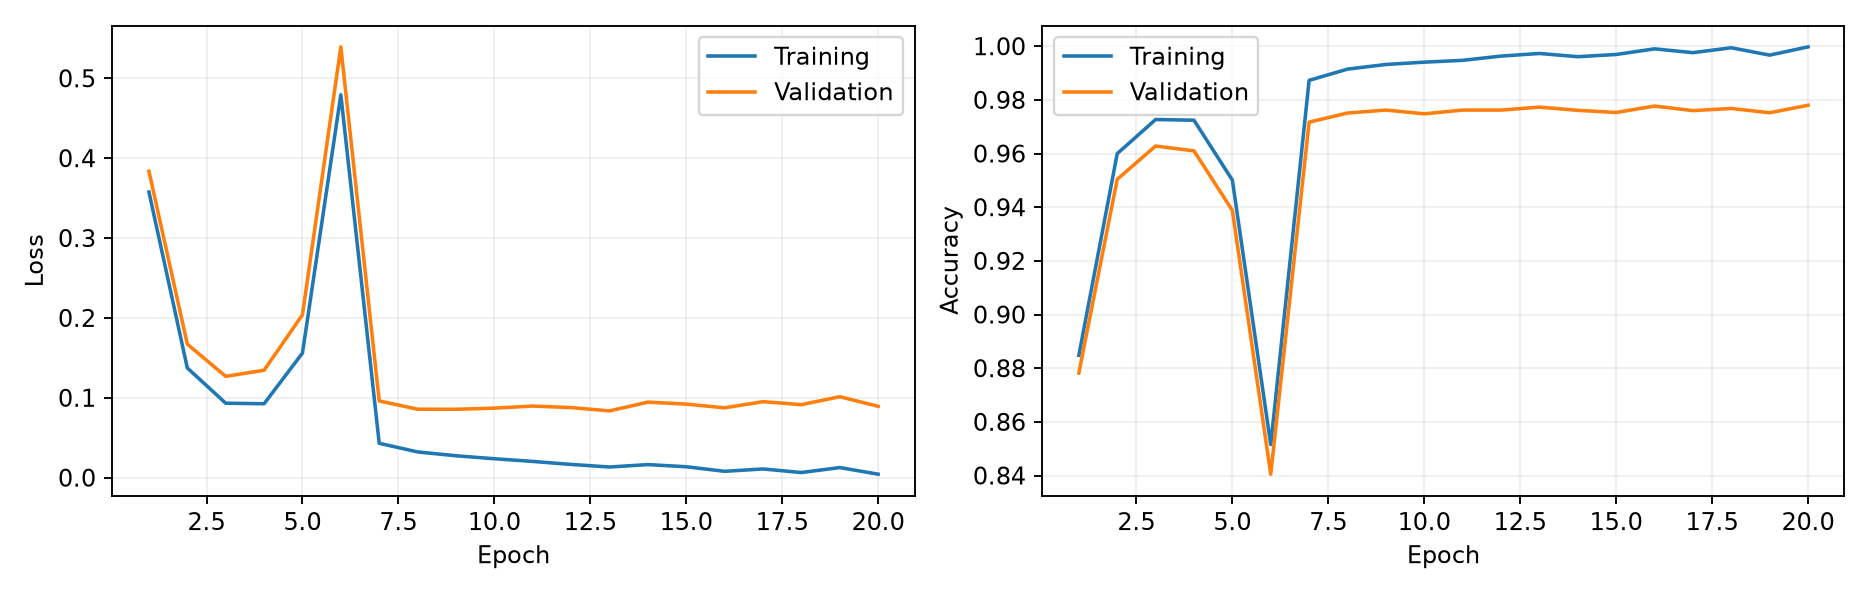
\includegraphics[width=.94\textwidth]{curves_en.png}\par\raggedright \begin{itemize}
\item On the left, lower loss is better; on the right, higher accuracy is better.
\item The model improves, but results fluctuate along the way.
\item Doing better on practice examples does not always mean doing better on new examples.
\end{itemize}

\note{Suggested speaking time: 80 seconds. Read the axes before discussing trends. Point to one curve at a time. Ask why we should look at validation as well as training. Use the gap to introduce overfitting as learning the practice data too specifically.}
\end{frame}

\begin{frame}{Our main result}
\begin{center}\begin{tabular}{lr}\toprule Official test result & Value\\\midrule Images evaluated & 10,000\\ Correct predictions & 9,790\\ Incorrect predictions & 210\\ Accuracy & 97.90\%\\ Macro F1 & 97.88\%\\\bottomrule\end{tabular}\end{center}\begin{itemize}
\item Accuracy is the proportion of correct predictions.
\item About 98 out of every 100 test images were classified correctly.
\end{itemize}

\note{Suggested speaking time: 65 seconds. Explain 9,790 divided by 10,000 before using the percentage. Macro F1 summarizes performance across digits while balancing precision and recall; keep this as a secondary indicator, not a formula exercise.}
\end{frame}

\begin{frame}{Which digits were confused?}
\centering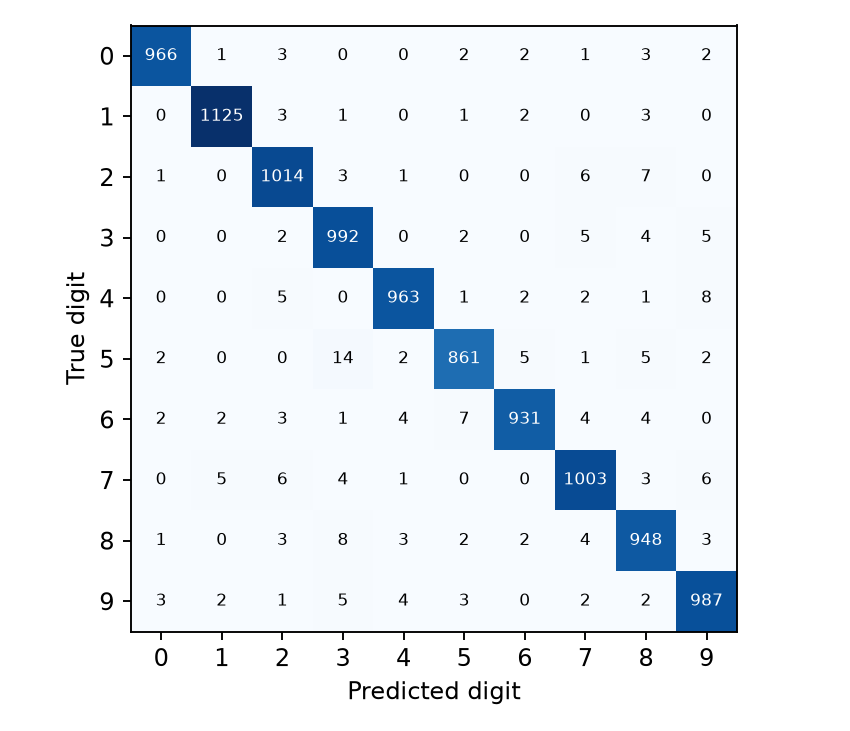
\includegraphics[height=.54\textheight]{confusion_en.png}\par\raggedright \begin{itemize}
\item Rows show the correct digit; columns show the predicted digit.
\item Counts on the main diagonal are correct answers.
\item The most common directed mistake was 5 predicted as 3: 14 cases.
\end{itemize}

\note{Suggested speaking time: 55 seconds. Show one correct cell and one incorrect cell. A confusion matrix breaks down the overall accuracy, showing where errors occur. Do not read every number.}
\end{frame}

\begin{frame}{Another check: separating one digit from the others}
\centering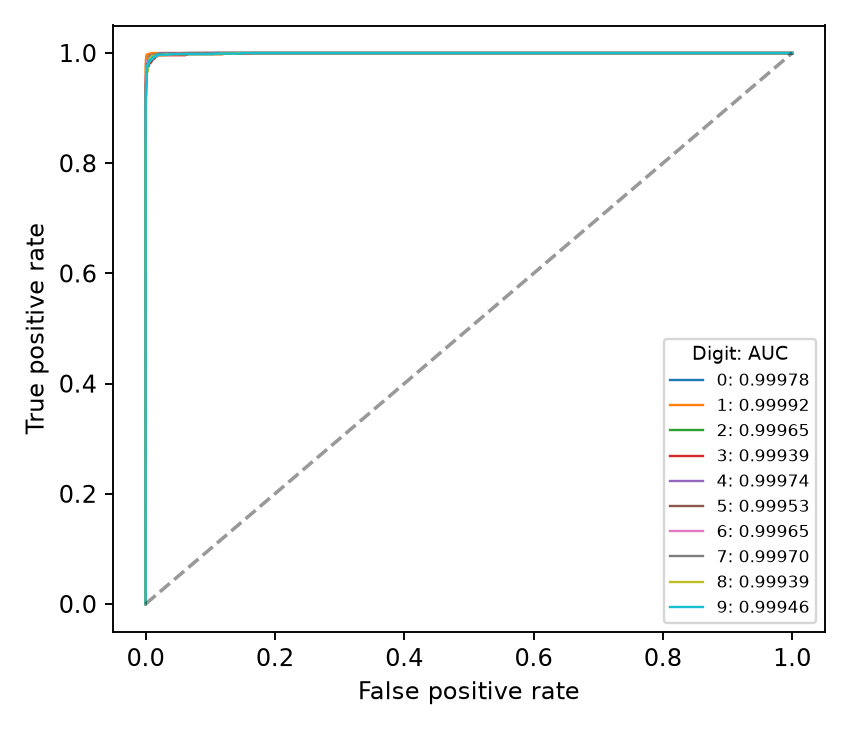
\includegraphics[height=.49\textheight]{roc_en.png}\par\raggedright \begin{itemize}
\item ROC shows the trade-off between detecting a digit and incorrectly accepting other digits.
\item AUC summarizes this separation: 0.5 is chance ranking and 1 is perfect ranking.
\item Our average AUC was about 0.9996; this is not a 99.96\% accuracy rate.
\end{itemize}

\note{Suggested speaking time: 65 seconds. Use digit 7 as an example and explain the axes as percentages of true sevens found and other digits accepted by mistake as sevens. We vary a score threshold. Focus on the intuition; averaging details and numerical integration are unnecessary.}
\end{frame}

\begin{frame}{The model can still make mistakes}
\centering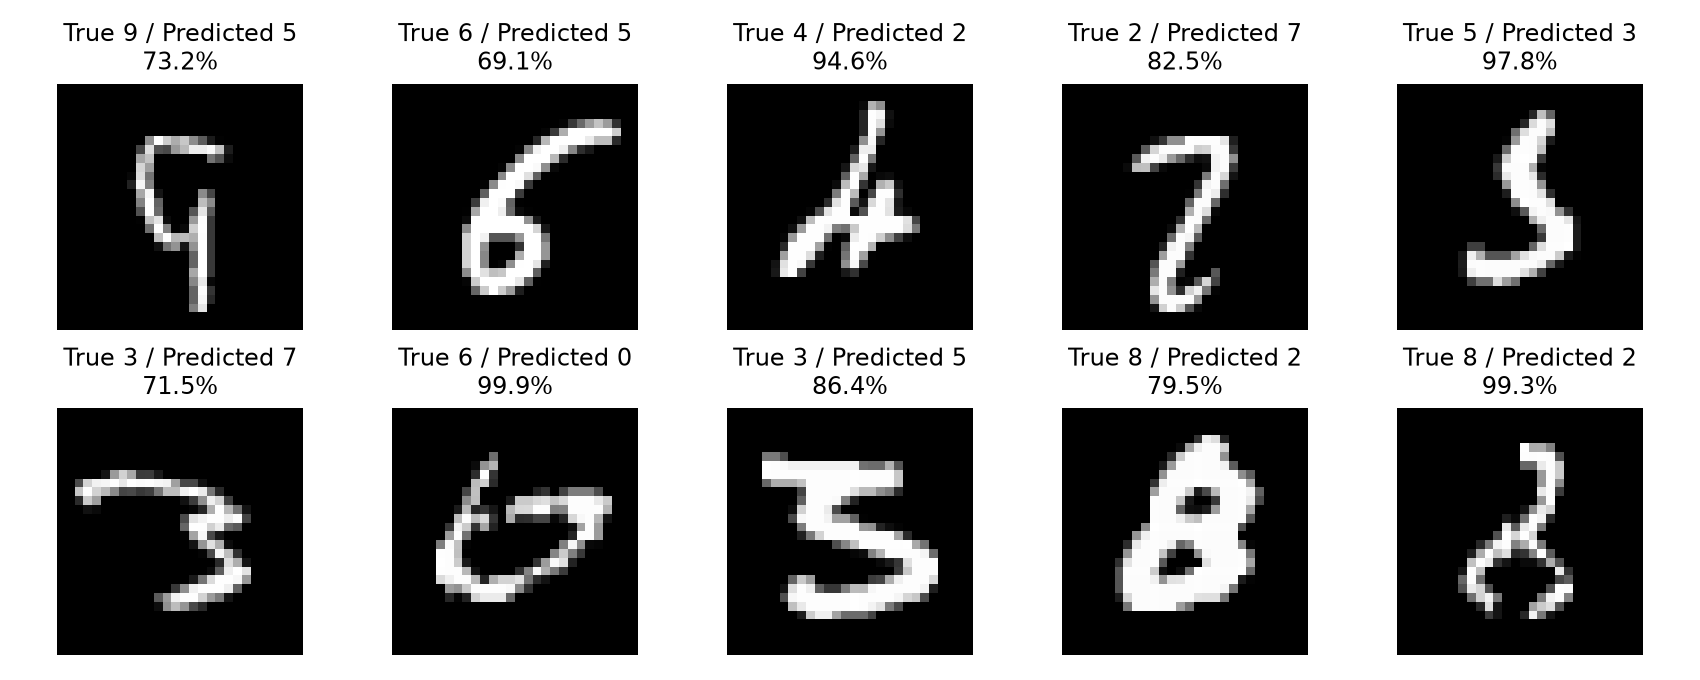
\includegraphics[width=.86\textwidth,height=.49\textheight,keepaspectratio]{errors_en.png}\par\raggedright \begin{itemize}
\item These are the first ten mistakes in the test data.
\item Some handwriting is ambiguous; other errors are limitations of the model.
\item A high score does not guarantee a correct answer.
\end{itemize}

\note{Suggested speaking time: 45 seconds. Ask the audience which example is hardest to read. Explain the displayed score as support assigned by this model to its chosen class, not certainty about the answer.}
\end{frame}

\begin{frame}{What we learned and what remains to explore}
\begin{itemize}
\item A network learns by repeating simple calculations and small adjustments.
\item Our recorded experiment achieved 97.90\% accuracy on the official test.
\item One successful run does not guarantee the same performance on every dataset or photograph.
\end{itemize}

\note{Suggested speaking time: 85 seconds. Mention that the implementation has 24 tests covering calculations and saved models. Future work would compare repeated runs and new handwriting conditions. Ask the audience to describe the learning cycle and reserve about three minutes for questions in the main talk.}
\end{frame}

\end{document}
